\documentclass[Naxsi]{subfiles}
\begin{document}
\section{Naxsi}
\label{sec:Naxsi}
Naxsi is written to be a fast, light and scalable \ac{WAF} for the Nginx web server. Naxsi means Nginx Anti Xss \& Sql Injection and it has a positive approach for network traffic inspection by using a white listing method. This means that traffic is blocked by default, and "good" traffic must be explicitly allowed. Naxsi uses two different files, which contain the rues. First, at the the server level configuration. Second, at the HTTP location level configuration. The first one is called the core rules, and it contains all characters and regular expressions that will increase the score of the request when the request has invalid content. The location level configuration has site specific rules and, thus allows for multiple virtual hosts. The local level configuration allows for each site to specify when a request should be dropped depending on the score the request is given by Naxsi.
The core level configuration is more or less a fixed list and, according to the Nginx website, it is not expected to evolve rapidly. On the other hand, the local level configuration is a site specific configuration, and thus needs to be created. Creating the rules is done by putting Naxsi in learning mode. When Naxsi is in learning mode, no request will be blocked, but rather it is seen as valid traffic and used for creating the whitelist rule set.

\subsection{Request flow}
When Naxsi is in production mode, it will actively give each request a score. Depending on the the local level configuration rule set, the request may be allowed or dropped. Figure \ref{fig:naxsi_flow} shows how logically each request is processed by Naxsi. First, the request is checked for "dangerous" symbols and SQL keywords. Second, the request is checked by the local level rules. Local level rules may overrule the core rules if configured such. Lastly, the request score is checked against the rule set. Depending on the score, the request is either blocked, which means the request gets forwarded to the DeniedURL, or the request is further processed.

\begin{figure}[h]
\caption{Naxsi request flow}
\centering
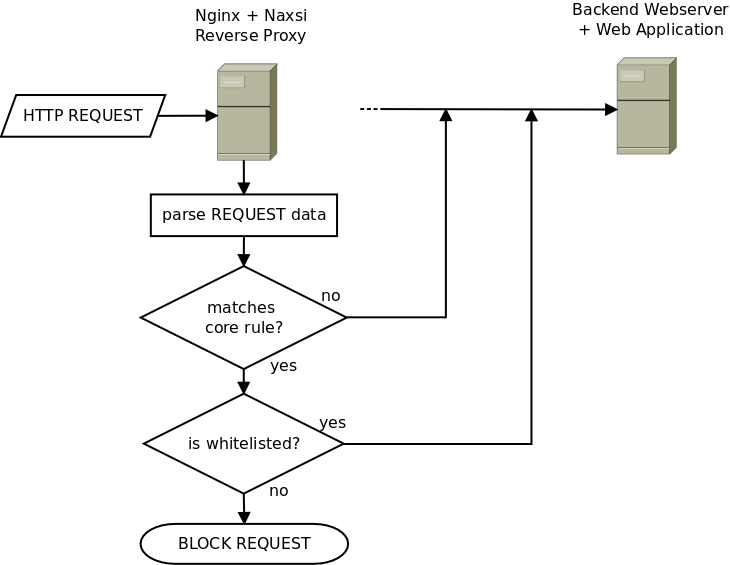
\includegraphics[width=0.75\textwidth] {images/request_flow.png}
\label{fig:naxsi_flow}
\end{figure}

\subsection{Whitelist processing}
\label{sec:naxsi_whitelist}
% From BUI: For whitelist processing, the process is the following : 1°) check rule X, 2°) if rule X is matched, look up in the various hashtables. hashtables are splitted according to "zones", to limit collisions (not handled by nginx's hashtable mechanism). you can find it in ngx_http_dummy_is_rule_whitelisted_n() from naxsi_runtime.c
%
%Technically, it is a third party nginx module, available as a package for many UNIX-like platforms. This module, by default, reads a small subset of simple rules (naxsi_core.rules) containing 99% of known patterns involved in websites vulnerabilities. For example, '<', '|' or 'drop' are not supposed to be part of a URI.
%Being very simple, those patterns may match legitimate queries, it is Naxsi's administrator duty to add specific rules that will whitelist those legitimate behaviours. The administrator can either add whitelists manually by analyzing nginx's error log, or (recommended) start the project by an intensive auto-learning phase that will automatically generate whitelisting rules regarding website's behaviour.
%In short, Naxsi behaves like a DROP-by-default firewall, the only job needed is to add required ACCEPT rules for the target website to work properly.
Naxsi has a small set of rules that can be referred to as blacklist, but in Naxsi terms are called \emph{core rules}. They contain regular expressions matching patterns that are often found in attacks.\\

\subsubsection*{Core Rules/blacklist}

\begin{verbatim}
MainRule "str:<" "msg:html open tag" "mz:ARGS|URL|BODY|$HEADERS_VAR:Cookie" "s:$XSS:8" id:1302; 
\end{verbatim}

\subsubsection*{Zones}

\subsubsection*{Whitlists}

\subsubsection*{Specific Rules}

\end{document}

